%%%%%%%%%%%%%%%%%%%%%%%%%%%%%%%%%%%%%%%%%%%%%%%%%%%%%%%%%%%%%%%%%%%%
%   	FILL OUT METADATA IN PREAMBLE TEX FILE FIRST
%%%%%%%%%%%%%%%%%%%%%%%%%%%%%%%%%%%%%%%%%%%%%%%%%%%%%%%%%%%%%%%%%%%%

%%%%%%%%%%%%%%%%%%%%%%%%%%%%%%%%%%%%%%%%%%%%%%%%%%%%%%%%%%%%%%%%%%%
%   LaTeX source code to approximate a NIST Technical report
%   CrossMark watermark will be added on final PDF
%   Developed by K. Miller, kmm5@nist.gov 
%   First release: 12-July-2023
%   Fixed lineno package syntax on 2-April-2024
%%%%%%%%%%%%%%%%%%%%%%%%%%%%%%%%%%%%%%%%%%%%%%%%%%%%%%%%%%%%%%%%%%%
%%%%%%%%%%%%%%%%%%%%%%%%%%%%%%%%%%%%%%%%%%%%%%%%%%%%%%%%%%%%%%%%%%%
%   Tagpdf settings, document class and template package 
%   DO NOT DELETE
\RequirePackage{pdfmanagement-testphase}
\DeclareDocumentMetadata{pdfversion=2.0,uncompress,testphase=phase-II}
\documentclass[12pt]{article}
\usepackage{settings}

%%%%%%%%%%%%%%%%%%%%%%%%%%%%%%%%%%%%%%%%%%%%%%%%%%%%%%%%%%%%%%%%%%%%%%%
% DRAFT: TRUE OR FALSE?
%%%%%%%%%%%%%%%%%%%%%%%%%%%%%%%%%%%%%%%%%%%%%%%%%%%%%%%%%%%%%%%%%%%%%%%
% REQUIRED!!! Select either Draft (toggletrue) or Final (togglefalse)
\newtoggle{draft}
% \toggletrue{draft} % use if this is a Draft
 \togglefalse{draft} % use if this is Final
%

\iftoggle{draft}{
\usepackage{lineno}
\linenumbers
}
{}



%%%%%%%%%%%%%%%%%%%%%%%%%%%%%%%%%%%%%%%%%%%%%%%%%%%%%%%%%%%%%%%%%%%%%%%
% Publication Metadata
%%%%%%%%%%%%%%%%%%%%%%%%%%%%%%%%%%%%%%%%%%%%%%%%%%%%%%%%%%%%%%%%%%%%%%%
\newcommand{\pubseries}{Series [Choose one from list]} % Replace with a series title from the list below %
% {Trustworthy and Responsible AI}
% {Advanced Manufacturing Series}
% {Creating Helpful Incentives to Produce Semiconductors for America}
% {Data Collection Instruments}
% {Economic Analysis Brief}
% {Grant/Contractor Report}
% {Handbook}
% {Interagency Report}
% {Internal Report}
% {National Standard Reference Data Series}
% {Special Publication 250}
% {Special Publication 260}
% {Special Publication 500}
% {Special Publication 1200}
% {Special Publication 1500}
% {Special Publication 1900}
% {Special Publication 2000}
% {Special Publication 2100}
% {Special Publication 2200}
% {Technical Note}
% {Technology Transfer Brief}
% {Voting Technology Series}
\newcommand{\pubnumber}{Publication Identifier} 
\newcommand{\DOI}{https://doi.org/10.6028/NIST.XXX.XXXX}
\newcommand{\pubmonth}{Month}
\newcommand{\pubyear}{Year}
\newcommand{\erratadate}{MM-DD-YYYY}
\newcommand{\pubtitle}{Title}
\newcommand{\pubsubtitle}{Subtitle} % delete if no subtitle %
%\newcommand{\draftstage}{Draft Stage} % Draft Stage is REQUIRED for drafts/preprints; Draft stages are listed in the NIST Publication Identifier guidance: https://www.nist.gov/nist-research-library/nist-technical-series-publications-author-instructions#pubid   %
\newcommand{\authorlist}{Author 1, Author 2, Author 3, Author 4, Author 5, Author 6, Author 7, Author 8, Author 9} % Format author name as: Last name First Initial Middle Initial (e.g., Miller KM)
\newcommand{\authorone}{Author 1}
\newcommand{\authortwo}{Author 2}
\newcommand{\authorthree}{Author 3}
\newcommand{\authorfour}{Author 4}
\newcommand{\authorfive}{Author 5}
\newcommand{\authorsix}{Author 6}
\newcommand{\authorseven}{Author 7}
\newcommand{\authoreight}{Author 8}
\newcommand{\authornine}{Author 9} % Add or delete commands based on number of authors %
\newcommand{\pubabstract}{REQUIRED. Concise, informative statement of the purpose, scope, methods, results, and conclusions/recommendations of the report. Do not include references. This section is required for indexing and cataloging purposes to assist with discoverability of the report.}
\newcommand{\keywords}{REQUIRED. Alphabetize, separate keywords with a semicolon, and end with a period.}
\newcommand{\publang}{English} %If translation, change to correct language%
\usepackage{pdfproperties}


%%Test macro from Ian Bell, NIST%%
%% \newcommand{\NISTsection}[2]{ \tagpdfparaOff \tagstructbegin{tag=H1}
%%\tagmcbegin{tag=H1}
%%\section{#1}
%%\tagmcend
%%\tagstructend
%%\label{#2}
%%\tagpdfparaOn
%%}
%\newcommand{\NISTsubsection}[2]{ \tagpdfparaOff \tagstructbegin{tag=H2}
%\tagmcbegin{tag=H2}
%\subsection{#1}
%\tagmcend
%\tagstructend
%\label{#2}
%\tagpdfparaOn
%}
%%%%%%%%%%%%%%%%%%%%%%%%%%%%%%%%%%%%%%%%%%%%%%%%%%%%%%%%%%%%%%%%%%%%
%   	PDF Tagging setup
%%%%%%%%%%%%%%%%%%%%%%%%%%%%%%%%%%%%%%%%%%%%%%%%%%%%%%%%%%%%%%%%%%%%
\tagpdfsetup
    {
      tabsorder=structure
    }

%%%%%%%%%%%%%%%%%%%%%%%%%%%%%%%%%%%%%%%%%%%%%%%%%%%%%%%%%%%%%%%%%%%%
%   	BEGIN DOCUMENT 
%%%%%%%%%%%%%%%%%%%%%%%%%%%%%%%%%%%%%%%%%%%%%%%%%%%%%%%%%%%%%%%%%%%%

\begin{document}

%%%%%%%%%%%%%%%%%%%%%%%%%%%%%%%%%%%%%%%%%%%%%%%%%%%%%%%%%%%%%%%%%%%%
%   	TAGPDF TIP - use \tagpdfparaOn and \tagpdfparaOff to turn paragraph tagging on and off 
%%%%%%%%%%%%%%%%%%%%%%%%%%%%%%%%%%%%%%%%%%%%%%%%%%%%%%%%%%%%%%%%%%%%
\tagpdfparaOn
%%%%%%%%%%%%%%%%%%%%%%%%%%%%%%%%%%%%%%%%%%%%%%%%%%%%%%%%%%%%%%%%%%%%
%   	READ and DELETE INSTRUCTIONS.TEX PAGE BEFORE SUBMISSION
%%%%%%%%%%%%%%%%%%%%%%%%%%%%%%%%%%%%%%%%%%%%%%%%%%%%%%%%%%%%%%%%%%%%

%%%%%%%%%%%%%%%%%%%%%%%%%%%%%%%%%%%%%%%%%%%%%%%%%%%%%%%%%%%%%%%%%%%%
%   Cover Page is REQUIRED and must contain the information 
%	displayed here, at a minimum. Additional artwork may be included 
%	(e.g., official project/conference logo, etc.).
%	Most info automated based on metadata entered in preamble.tex
%%%%%%%%%%%%%%%%%%%%%%%%%%%%%%%%%%%%%%%%%%%%%%%%%%%%%%%%%%%%%%%%%%%%
	\begin{titlepage}
		\begin{flushright}
%%%%%%%%%%%%%%%%%%%%%%%%%%%%%%%%%%%%%%%%%%%%%%%%%%%%%%%%%%%%%%%%%%%%
% 	Automated based on metadata in preamble.tex
%%%%%%%%%%%%%%%%%%%%%%%%%%%%%%%%%%%%%%%%%%%%%%%%%%%%%%%%%%%%%%%%%%%%
\tagpdfparaOff
%%%%%%%%%%%%%%%%%%%%%%%%%%%%%%%%%%%%%%%%%%%%%%%%%%%%%%%%%%%%%%%%%%%%
%   	TAGPDF TIP - use \tagstructbegin \tagmcbegin \tagmcend 
%       \tagstructend around section headings.     
%%%%%%%%%%%%%%%%%%%%%%%%%%%%%%%%%%%%%%%%%%%%%%%%%%%%%%%%%%%%%%%%%%%%
\tagstructbegin{tag=H} %start heading tag
 \tagmcbegin{tag=H} % start heading content
 
\LARGE{\textbf{NIST \pubseries}}\\
\LARGE{\textbf{\pubnumber}}\\

\tagmcend % end heading content
 \tagstructend % end heading tag
 
\vfill

\tagstructbegin{tag=H} %start heading tag
 \tagmcbegin{tag=H} % start heading content
 
\Huge{\textbf{\pubtitle}}\\

\tagmcend % end heading content
 \tagstructend % end heading tag

 \tagstructbegin{tag=H} %start heading tag
 \tagmcbegin{tag=H} % start heading content
 
\Large{\textit{\pubsubtitle}}\\

\tagmcend % end heading content
 \tagstructend % end heading tag
%%%%%%%%%%%%%%%%%%%%%%%%%%%%%%%%%%%%%%%%%%%%%%%%%%%%%%%%%%%%%%%%%%%%
%   	TAGPDF TIP - remember to turn on paragraph tagging after
%       section headings     
%%%%%%%%%%%%%%%%%%%%%%%%%%%%%%%%%%%%%%%%%%%%%%%%%%%%%%%%%%%%%%%%%%%%
\tagpdfparaOn 
% Include below if this is a draft
%\vfill 
%\Large{\draftstage}\\ 
\vfill
%%%%%%%%%%%%%%%%%%%%%%%%%%%%%%%%%%%%%%%%%%%%%%%%%%%%%%%%%%%%%%%%%%%%
%	Authors - automated based on metadata in preamble.tex
%%%%%%%%%%%%%%%%%%%%%%%%%%%%%%%%%%%%%%%%%%%%%%%%%%%%%%%%%%%%%%%%%%%%
\large \authorone\\
\large \authortwo\\
\large \authorthree\\
\large \authorfour\\
\large \authorfive\\
\large \authorsix\\
\large \authorseven\\
\large \authoreight\\
\large \authornine\\
\vfill
%%%%%%%%%%%%%%%%%%%%%%%%%%%%%%%%%%%%%%%%%%%%%%%%%%%%%%%%%%%%%%%%%%%%
%	The DOI is automated based on metadata in preamble.tex	
%%%%%%%%%%%%%%%%%%%%%%%%%%%%%%%%%%%%%%%%%%%%%%%%%%%%%%%%%%%%%%%%%%%%
\normalsize This publication is available free of charge from:\\
\DOI\\
\vfill
%%%%%%%%%%%%%%%%%%%%%%%%%%%%%%%%%%%%%%%%%%%%%%%%%%%%%%%%%%%%%%%%%%%%
%	USE FOR SP 1900 PUBLICATIONS; SEE SETTINGS.STY FILE	
%%%%%%%%%%%%%%%%%%%%%%%%%%%%%%%%%%%%%%%%%%%%%%%%%%%%%%%%%%%%%%%%%%%%
% \lsstyle
% \hrule
% \vspace{3pt}
% \LARGE{CYBER-PHYSICAL  SYSTEMS}
% \vspace{6pt}
% \hrule
% \vfill
%%%%%%%%%%%%%%%%%%%%%%%%%%%%%%%%%%%%%%%%%%%%%%%%%%%%%%%%%%%%%%%%%%%%
%	NIST LOGO - keep as-is The cover page can include additional visual elements. Commercial logos are not permitted. NIST program logos are permitted. Other agency logos are permitted if interagency report.
%%%%%%%%%%%%%%%%%%%%%%%%%%%%%%%%%%%%%%%%%%%%%%%%%%%%%%%%%%%%%%%%%%%%
 \tagpdfparaOff \tagstructbegin{tag=Figure,alttext={NIST logo}}%
\tagmcbegin{tag=Figure}%


\includegraphics[trim=0 0 0.7in 0,clip,width=4in]{NIST-logo.png}\\ 

  \tagmcend
 \tagstructend
 
\end{flushright}
\end{titlepage}
\begin{titlepage}
%%%%%%%%%%%%%%%%%%%%%%%%%%%%%%%%%%%%%%%%%%%%%%%%%%%%%%%%%%%%%%%%%%%%
%	Title Page is REQUIRED
%%%%%%%%%%%%%%%%%%%%%%%%%%%%%%%%%%%%%%%%%%%%%%%%%%%%%%%%%%%%%%%%%%%%
\begin{flushright}
%%%%%%%%%%%%%%%%%%%%%%%%%%%%%%%%%%%%%%%%%%%%%%%%%%%%%%%%%%%%%%%%%%%%
%   Automated based on metadata in preamble.tex
%%%%%%%%%%%%%%%%%%%%%%%%%%%%%%%%%%%%%%%%%%%%%%%%%%%%%%%%%%%%%%%%%%%%
%%%%%%%%%%%%%%%%%%%%%%%%%%%%%%%%%%%%%%%%%%%%%%%%%%%%%%%%%%%%%%%%%%%%
%   	TAGPDF TIP - turn on or off paragraph tagging for each 
%       page or section  
%%%%%%%%%%%%%%%%%%%%%%%%%%%%%%%%%%%%%%%%%%%%%%%%%%%%%%%%%%%%%%%%%%%%
\tagpdfparaOff \tagstructbegin{tag=H} %start heading struc
 \tagmcbegin{tag=H} % start heading mc
\LARGE{\textbf{NIST \pubseries}}\\
\LARGE{\textbf{\pubnumber}}\\
\tagmcend % end heading mc
 \tagstructend % end heading struc
\vfill
\tagpdfparaOff \tagstructbegin{tag=H} %start heading struc
 \tagmcbegin{tag=H} % start heading mc
\Huge{\textbf{\pubtitle}}\\
\tagmcend % end heading mc
 \tagstructend % end heading struc
 
 \tagpdfparaOff \tagstructbegin{tag=H} %start heading struc
 \tagmcbegin{tag=H} % start heading mc
\Large{\textit{\pubsubtitle}}\\
\tagmcend % end heading mc
 \tagstructend % end heading struc
 
\tagpdfparaOn
%include if draft
%\vfill 
%\Large{\draftstage}
\vfill
%%%%%%%%%%%%%%%%%%%%%%%%%%%%%%%%%%%%%%%%%%%%%%%%%%%%%%%%%%%%%%%%%%%%
%	Author Order and Grouping. Always identify the primary author/creator first (s/he does not have to be a NIST author). For publications with multiple authors, group authors by their organizational affiliation. The organizational groupings and the names within each grouping should generally be ordered by decreasing level of contribution.
%	For non-NIST authors, list their city and state below their organization name.
%	For NIST authors, include the Division and Laboratory names (but do not include their city and state).
%%%%%%%%%%%%%%%%%%%%%%%%%%%%%%%%%%%%%%%%%%%%%%%%%%%%%%%%%%%%%%%%%%%%
\normalsize \authorone\\
\authortwo\\
\authorthree\\
\authorfour\\
\textit{Office of XXXX}\\
\textit{First Operating Unit}\\
\vspace{12pt}
\authorfive\\
\authorsix\\
\authorseven\\
\textit{Office of XXXX}\\
\textit{Second Operating Unit}\\
\vspace{12pt}
\authoreight\\
\authornine\\
\textit{Office of XXXX}\\
\textit{Second Operating Unit}\\
\vfill
%%%%%%%%%%%%%%%%%%%%%%%%%%%%%%%%%%%%%%%%%%%%%%%%%%%%%%%%%%%%%%%%%%%%
%   Automated based on metadata in preamble.tex
%%%%%%%%%%%%%%%%%%%%%%%%%%%%%%%%%%%%%%%%%%%%%%%%%%%%%%%%%%%%%%%%%%%%
\normalsize This publication is available free of charge from:\\
\DOI\\
\vfill
\normalsize \pubmonth~\pubyear\\
%\textsc{Includes Updates as of \erratadate; See \appendixname~\ref{app:log}} %include if errata update

\vfill
%%%%%%%%%%%%%%%%%%%%%%%%%%%%%%%%%%%%%%%%%%%%%%%%%%%%%%%%%%%%%%%%%%%%
%  Department of Commerce LOGO - leave as-is
%%%%%%%%%%%%%%%%%%%%%%%%%%%%%%%%%%%%%%%%%%%%%%%%%%%%%%%%%%%%%%%%%%%%
\tagpdfparaOff \tagstructbegin{tag=Figure,alttext={Department of Commerce logo}}%
\tagmcbegin{tag=Figure}%


\includegraphics[width=0.2\linewidth]{DoC-logo.pdf}\\ 

  \tagmcend
 \tagstructend
 \tagpdfparaOn
\vfill
%%%%%%%%%%%%%%%%%%%%%%%%%%%%%%%%%%%%%%%%%%%%%%%%%%%%%%%%%%%%%%%%%%%%
%  Department of Commerce & NIST Leadership 
%	will be updated as changes occur
%%%%%%%%%%%%%%%%%%%%%%%%%%%%%%%%%%%%%%%%%%%%%%%%%%%%%%%%%%%%%%%%%%%%
\footnotesize U.S. Department of Commerce\\ 
\textit{Gina M. Raimondo, Secretary}\\
\vspace{10pt}
National Institute of Standards and Technology\\ 
\hspace*{-3cm}\textit{Laurie E. Locascio, NIST Director and Under Secretary of Commerce for Standards and Technology}  

\end{flushright}

\end{titlepage}
%%%%%%%%%%%%%%%%%%%%%%%%%%%%%%%%%%%%%%%%%%%%%%%%%%%%%%%%%%%%%%%%%%%%
%   Disclaimer & Publication History Page -- REQUIRED
%%%%%%%%%%%%%%%%%%%%%%%%%%%%%%%%%%%%%%%%%%%%%%%%%%%%%%%%%%%%%%%%%%%%
\begin{titlepage}

\begin{flushleft}
\tagpdfparaOn
\footnotesize  Certain equipment, instruments, software, or materials, commercial or non-commercial, are identified in this paper in order to specify the experimental procedure adequately. Such identification does not imply recommendation or endorsement of any product or service by NIST, nor does it imply that the materials or equipment identified are necessarily the best available for the purpose.\\ 
%%%%%%%%%%%%%%%%%%%%%%%%%%%%%%%%%%%%%%%%%%%%%%%%%%%%%%%%%%%%%%%%%%%%
% OTHER DISCLAIMERS - INCLUDE AS APPROPRIATE %
%%%%%%%%%%%%%%%%%%%%%%%%%%%%%%%%%%%%%%%%%%%%%%%%%%%%%%%%%%%%%%%%%%%%
% This publication was produced as part of contract <contract number> with the National Institute of Standards and Technology. The contents of this publication do not necessarily reflect the views or policies of the National Institute of Standards and Technology or the US Government.
% The NIST Data Collection Instruments series include questionnaires or survey instruments, interview guides, and other structured means of collecting data. Some of these instruments are designed for human subjects research focused on households, social institutions, and businesses. The instruments are approved by both NIST Institutional Review Board (IRB) and OMB/Paperwork Reduction Act.
% Publications in the SP 1200 subseries include written procedural methods in the design and implementation of experiments that ensure successful replication of results by others. Publications may include detailed procedures, lists of required equipment and instruments, information on safety precautions, the calculation of results and reporting standards.
% Publications in the SP1500 subseries are intended to capture external perspectives related to NIST standards, measurement, and testing-related efforts. These external perspectives can come from industry, academia, government, and others. These reports are intended to document external perspectives and do not represent official NIST positions. The opinions, recommendations, findings, and conclusions in this publication do not necessarily reflect the views or policies of NIST or the United States Government.
% Publications in the SP 2000 subseries provide detailed descriptions of important activities and features related to the use and harmonization of standards and conformity assessment in the United States and globally. The publications include reports, guidelines, and other information resources on key concepts, activities, features, and other specific topics regarding coordination of standards and use of conformity assessment impacting both international and U.S. trade.
% Publications in the SP 2100 subseries are proceedings from conferences organized predominately by NIST scientific and technical staff. These proceedings are published as a single document that includes all abstracts or extended abstracts accepted by the conference organizers. This publication may include external perspectives from industry, academia, government, and others. The opinions, recommendations, findings, and conclusions in this publication do not necessarily reflect the views or policies of NIST or the United States Government.
\vfill
%%%%%%%%%%%%%%%%%%%%%%%%%%%%%%%%%%%%%%%%%%%%%%%%%%%%%%%%%%%%%%%%%%%%
%   This section maintained by Library - do not change
%%%%%%%%%%%%%%%%%%%%%%%%%%%%%%%%%%%%%%%%%%%%%%%%%%%%%%%%%%%%%%%%%%%%
\footnotesize 
{\textbf{NIST Technical Series Policies}}\\
{\href{https://doi.org/10.6028/NIST-TECHPUBS.CROSSMARK-POLICY}{Copyright, Use, and Licensing Statements}\\
\href{https://www.nist.gov/nist-research-library/nist-technical-series-publications-author-instructions#pubid}{NIST Technical Series Publication Identifier Syntax}}
\vfill
%%%%%%%%%%%%%%%%%%%%%%%%%%%%%%%%%%%%%%%%%%%%%%%%%%%%%%%%%%%%%%%%%%%%
%  Complete this section as appropriate
% ERB approval date is REQUIRED.
% Publication ID, Month/Year, and DOI of report being replaced (superseded)  is only required if this manuscript is a new version (revision, edition, errata update). 
%%%%%%%%%%%%%%%%%%%%%%%%%%%%%%%%%%%%%%%%%%%%%%%%%%%%%%%%%%%%%%%%%%%%
{\textbf{Publication History}}\\
Approved by the NIST Editorial Review Board on YYYY-MM-DD\\
Supersedes NIST Series XXX (Month Year) DOI\\
\vfill
%%%%%%%%%%%%%%%%%%%%%%%%%%%%%%%%%%%%%%%%%%%%%%%%%%%%%%%%%%%%%%%%%%%%
% This section is automated from metadata in preamble.tex
%%%%%%%%%%%%%%%%%%%%%%%%%%%%%%%%%%%%%%%%%%%%%%%%%%%%%%%%%%%%%%%%%%%%
{\textbf{How to cite this NIST Technical Series Publication:}} \\
 \authorlist~(\pubyear)~\pubtitle.~(National Institute of Standards and Technology, Gaithersburg, MD),~\pubnumber.~ \DOI
\vfill
%%%%%%%%%%%%%%%%%%%%%%%%%%%%%%%%%%%%%%%%%%%%%%%%%%%%%%%%%%%%%%%%%%%%
% ORCID iDs are REQUIRED for all NIST employees. 
% External author ORCID iDs are optional.
% See NIST Directive O 1801.00 for more details.

%%%%%%%%%%%%%%%%%%%%%%%%%%%%%%%%%%%%%%%%%%%%%%%%%%%%%%%%%%%%%%%%%%%%
{\textbf{Author ORCID iDs}}\\
 \authorone: 0000-0000-0000-0000\\
\authortwo: 0000-0000-0000-0000\\
\authorthree: 0000-0000-0000-0000\\
\authorfour: 0000-0000-0000-0000\\
\vfill
%%%%%%%%%%%%%%%%%%%%%%%%%%%%%%%%%%%%%%%%%%%%%%%%%%%%%%%%%%%%%%%%%%%%
% OPTIONAL, include email address / mailing address / etc.
%%%%%%%%%%%%%%%%%%%%%%%%%%%%%%%%%%%%%%%%%%%%%%%%%%%%%%%%%%%%%%%%%%%%
{\textbf{Contact Information}}\\
{\href{mailto:contact@nist.gov}{contact@nist.gov}}
\vfill
%%%%%%%%%%%%%%%%%%%%%%%%%%%%%%%%%%%%%%%%%%%%%%%%%%%%%%%%%%%%%%%%%%%%
% OPTIONAL FOR DRAFTS, include how to submit comments and any other relevant information (e.g., disclaimers or FOIA release statements). 
%%%%%%%%%%%%%%%%%%%%%%%%%%%%%%%%%%%%%%%%%%%%%%%%%%%%%%%%%%%%%%%%%%%%
{\textbf{Public Comment Period}}\\
Month Day, YYYY – Month Day, YYYY

{\textbf{Submit Comments}}\\ 
{\href{mailto:contact@nist.gov}{contact@nist.gov}} \\
Mailing Address

\end{flushleft}


\end{titlepage}
%%%%%%%%%%%%%%%%%%%%%%%%%%%%%%%%%%%%%%%%%%%%%%%%%%%%%%%%%%%%%%%%%%%%
%   Start front matter - page number starts with "i"
% Additional information can be added to the verso and front matter as needed
%%%%%%%%%%%%%%%%%%%%%%%%%%%%%%%%%%%%%%%%%%%%%%%%%%%%%%%%%%%%%%%%%%%%
\begin{titlepage}
\pagenumbering{roman}
\thispagestyle{fancy}
\renewcommand{\headrulewidth}{0pt}

\ExplSyntaxOn
 \tagmcbegin{artifact=pagination/header}
 \fancyhead{}
  \fancyhead[l]{\small \pubnumber \\ 
	\small \pubmonth \pubyear \\}
	\fancyfoot[c]{\thepage}
  \tagmcend
\ExplSyntaxOff

  \tagpdfparaOff \tagstructbegin{tag=H} %start heading struc
 \tagmcbegin{tag=H} % start heading mc
\section*{Abstract}
 \tagmcend % end heading mc
 \tagstructend % end heading struc
 \tagpdfparaOn
\pubabstract


   \tagpdfparaOff \tagstructbegin{tag=H} %start heading struc
 \tagmcbegin{tag=H} % start heading mc
\section*{Keywords}
 \tagmcend % end heading mc
 \tagstructend % end heading struc
 \tagpdfparaOn
\keywords


\newpage
%%%%%%%%%%%%%%%%%%%%%%%%%%%%%%%%%%%%%%%%%%%%%%%%%%%%%%%%%%%%%%%%%%%%
%   Table of Contents is required
% 	List of Tables & Figures required if more than 5 tables/figures
%   TagPDF does not recognize TOC in the PDF, will tag each entry as 
%   a paragraph
%%%%%%%%%%%%%%%%%%%%%%%%%%%%%%%%%%%%%%%%%%%%%%%%%%%%%%%%%%%%%%%%%%%%
 \tagpdfparaOff
\ExplSyntaxOn
 \tagmcbegin{artifact=pagination/header}
\vspace*{-3cm}\small{\pubnumber \newline  \pubmonth~\pubyear}
\vspace{18pt}
  \tagmcend
\ExplSyntaxOff


\begin{center}
{
\hypersetup{ linkcolor = {black}}
	\tableofcontents
	\appendixtitleon
    \appendixtitletocon
	\listoftables
	\listoffigures
 }
	\end{center}

\pagebreak
%%%%%%%%%%%%%%%%%%%%%%%%%%%%%%%%%%%%%%%%%%%%%%%%%%%%%%%%%%%%%%%%%%%%
%   Front matter continued
%%%%%%%%%%%%%%%%%%%%%%%%%%%%%%%%%%%%%%%%%%%%%%%%%%%%%%%%%%%%%%%%%%%%
\thispagestyle{fancy}
\renewcommand{\headrulewidth}{0pt}
\ExplSyntaxOn
 \tagmcbegin{artifact=pagination/header}
  \fancyhead{}
  \fancyhead[l]{\small \pubnumber \\ 
	\small \pubmonth~\pubyear \\}
	\fancyfoot[c]{\thepage}
  \tagmcend
\ExplSyntaxOff

 \tagpdfparaOff \tagstructbegin{tag=H1} 
 \tagmcbegin{tag=H1} 
\section*{Foreword}
 \tagmcend
 \tagstructend
 \tagpdfparaOn
OPTIONAL. The foreword is an introductory statement that presents background material or places the report in context. It is usually written by someone other than the creator of the report. The name and affiliation of the foreword author should be listed.
 
 \tagpdfparaOff \tagstructbegin{tag=H1}
 \tagmcbegin{tag=H1} 
\section*{Preface}
\tagmcend
 \tagstructend
 \tagpdfparaOn
OPTIONAL. A preface is an introductory statement that announces the purpose and scope of the report and may acknowledge contributions of those not listed as authors. Material that is not necessary for understanding the report belongs in the preface. 
 
 \tagpdfparaOff \tagstructbegin{tag=H1}
 \tagmcbegin{tag=H1} %avoid page break!
\section*{Acknowledgments}
\tagmcend
 \tagstructend
 \tagpdfparaOn
OPTIONAL. Delete if not needed.
 
 \tagpdfparaOff \tagstructbegin{tag=H1}
 \tagmcbegin{tag=H1} 
\section*{Author Contributions}
\tagmcend
 \tagstructend
\tagpdfparaOn
% OPTIONAL: Provide statement on the contributions of each author using the ANSI/NISO Z39.104-2022 CRediT roles taxonomy. This can also be used to inform the sequence of authors on the cover page and in the citation (i.e., authors with more roles are listed first).

\textbf{\authorone}: Conceptualization, Methodology, Software. \textbf{\authortwo}: Data curation, Writing- Original draft preparation. \textbf{\authorthree}: Visualization, Investigation. \textbf{\authorfour}: Supervision. \textbf{\authorfive}: Software, Validation. \textbf{\authorsix}: Writing- Reviewing and Editing.
 

\end{titlepage}
%%%%%%%%%%%%%%%%%%%%%%%%%%%%%%%%%%%%%%%%%%%%%%%%%%%%%%%%%%%%%%%%%%%%
%   Header text and page numbering
%%%%%%%%%%%%%%%%%%%%%%%%%%%%%%%%%%%%%%%%%%%%%%%%%%%%%%%%%%%%%%%%%%%%
\pagestyle{fancy}
\renewcommand{\headrulewidth}{0pt}
\ExplSyntaxOn
 \tagmcbegin{artifact=pagination/header}
  \fancyhead{}
  \fancyhead[l]{\small \pubnumber \\ 
	\small \pubmonth~\pubyear \\}
   \fancyhead[r]{\small {[ShortTitle1]} \\ 
	\small {[ShortTitle2]} \\}
   \tagmcend
\ExplSyntaxOff
\pagenumbering{arabic}
%%%%%%%%%%%%%%%%%%%%%%%%%%%%%%%%%%%%%%%%%%%%%%%%%%%%%%%%%%%%%%%%%%%%
%   Start body of text - page number starts with "1"
%%%%%%%%%%%%%%%%%%%%%%%%%%%%%%%%%%%%%%%%%%%%%%%%%%%%%%%%%%%%%%%%%%%%

 \tagpdfparaOff \tagstructbegin{tag=H1}
 \tagmcbegin{tag=H1} 
\section*{Executive Summary}
\tagmcend
 \tagstructend
 \addcontentsline{toc}{section}{Executive Summary}
\label{sec:es}
\tagpdfparaOn
\normalsize OPTIONAL. Recommended if report exceeds 50 pages. Non-technical presentation that provides information to management and/or decision-makers who need a basic understanding of the findings and recommendations. May include any policy or fiscal implications of the recommendations.
\newpage
 \tagpdfparaOff \tagstructbegin{tag=H1}
 \tagmcbegin{tag=H1}
% Macro from Ian Bell, NIST
% \NISTsection{Section 1}{sec:intro}
\section{Section 1}
\tagmcend
 \tagstructend
 
\label{sec:intro}
\tagpdfparaOn
\normalsize 
Use the appropriate list style for all lists. An example of an unordered list:
\begin{itemize}
    \item[$\bullet$]  This is a bulleted list
    \begin{itemize}
        \item[$\circ$] This is a a level two bullet
        \begin{itemize}
        \item[$\--$]  This is a a level three bullet
    \end{itemize}
    \end{itemize}
\end{itemize}

An example of an ordered list:
\begin{enumerate}
    \item The first step is to decide how you want to order the list
    \item Apply the correct style
\end{enumerate}

When referring to references in the text parenthetically, use the form [X]. For example: 
\begin{quote}
As Jones and Smith have shown in [X]… 
\end{quote}
However, when a reference is referred to non-parenthetically, use the form Ref. \cite{Caxton,Eston1993,Farindon,FIPS1402,giancoli2008physics,Isley,Joslin,Maloney2016,MSU-CSE-06-2,Prives2016,Roberts1982,SP80053r4,Xiong2015}, except at the beginning of a sentence where Reference [X] is the correct form.

 \tagpdfparaOff \tagstructbegin{tag=H2}
 \tagmcbegin{tag=H2}
\subsection{Section 1.1.}
\tagmcend
 \tagstructend
 \label{level2:headingscap}
\tagpdfparaOn
All sections and subsection titles should be capitalized. Here is an example of a text box, use these sparingly.\tagpdfparaOff
\footnote{Disclaimer needs to appear as a numbered footnote at first mention of commercial product}

 \tagstructbegin{tag=Div}
\tagmcbegin{tag=Div}
\begin{tcolorbox}%[before upper=\tagpdfparaOn]
This is some block text. You can change the spacing, background color, and font formatting as needed
\end{tcolorbox}
\tagmcend
\tagstructend

 \tagpdfparaOff \tagstructbegin{tag=H3}
 \tagmcbegin{tag=H3}
\subsubsection{Section 1.1.1.}
\tagmcend
 \tagstructend
\label{level3:headingscap}
\tagpdfparaOn
Section references are Sec. X. Section X is used at beginning of sentence.
Tables should appear after they are mentioned in the text (see Table~\ref{tab:example}). 

 
\begin{table}[h]
\tagpdfparaOff \tagstructbegin{tag=Table}
 \tagmcbegin{tag=Table}
	\centering
	\caption{Title.}
	\label{tab:example}
	\small
	\begin{tabular}{cc}
		\hline
		ColumnA & ColumnB \\ \hline
		text & text{\scriptsize $^{\rm a}$} \\
		text & text \\
		text & text \\
		text & text \\
		\hline
	\end{tabular}
	
	{\footnotesize 	{\scriptsize $^{\rm a}$}Footnote}
\tagmcend
\tagstructend
\end{table}
Manuscripts must comply with the NIST policy on the use of the International System of Units (SI). See:
\begin{itemize}
    \item[$\bullet$] NIST Special Publication 811, 2008 Edition, Guide for the Use of the International System of Units (SI), by A. Thompson and B. N. Taylor at \href{https://www.nist.gov/pml/special-publication-811}{https://www.nist.gov/pml/special-publication-811}
\end{itemize}
They must also comply with the NIST policy on statements of uncertainty associated with measurement results. See:
\begin{itemize}
    \item[$\bullet$] NIST Technical Note 1297, 1994 Edition, Guidelines for Evaluating and Expressing the Uncertainty of NIST Measurement Results, by B. N. Taylor and C. E. Kuyatt at \href{https://www.nist.gov/pml/nist-technical-note-1297}{https://www.nist.gov/pml/nist-technical-note-1297}
\end{itemize}

 \tagstructbegin{tag=H4}
 \tagmcbegin{tag=H4}
\paragraph{Section 1.1.1.1.}
\tagmcend
 \tagstructend
 \tagpdfparaOn
Equation references are Eq. (X). Equation (X) is used at beginning of sentence.
 
\tagpdfparaOff 
\begin{equation}
\tagstructbegin{tag=Formula}
 \tagmcbegin{tag=Formula}
\label{eq:example}
{x}^{n} + {y}^{n} = {z}^{n}
\tagmcend
\tagstructend
\end{equation}

\tagpdfparaOn
 
The default table style (borders, shading, banding, size) can be adjusted as needed. Any use of color in tables must not be used to convey information and must pass \href{https://support.microsoft.com/en-us/office/make-your-content-accessible-to-everyone-with-the-accessibility-checker-38059c2d-45ef-4830-9797-618f0e96f3ab}{contrast validation}. Authors should avoid merging table cells or using tables to achieve text formats. Use simple table structures, specify column header information, and repeating header rows. Superscripted letters (a, b, c, etc.) should be used for table footnotes and should appear directly below the table, restarting with ‘a’ for each table.

Figures should not rely on color alone to convey information. When choosing color follow these best practices: provide sufficient contrast, avoid \href{https://www.nature.com/articles/519291d}{rainbow scale}, and check your color palettes using \href{http://selection.datavisualization.ch/}{online tools}.

All images must have alternative text. The text should explain the image for those who use screen readers. The goal is to simplify complex images where possible. Follow instructions on how to add alt text to images in the \href{https://helpx.adobe.com/acrobat/using/editing-document-structure-content-tags.html#add_alternate_text_and_supplementary_information_to_tags}{PDF} or tagging figures with alttext using TagPDF.

Figure references are written as Fig. X. Figure X is used as the beginning of a sentence. Figures should appear after they are mentioned in the text. 

The alt text used for \href{https://equidox.co/blog/beyond-basic-alt-text-charts-maps-and-diagrams/}{Fig. \ref{fig:cellphone} } is “Line graph showing an upward trend in cell phone services from 2001 through 2010, with a corresponding downward trend in residential phone services over the same period.” 
 

\begin{figure}[H] 

 \tagpdfparaOff \tagstructbegin{tag=Figure,alttext={Line graph showing an upward trend in cell phone services from 2001 through 2010, with a corresponding downward trend in residential phone services over the same period}}%
\tagmcbegin{tag=Figure}%
	\centering 	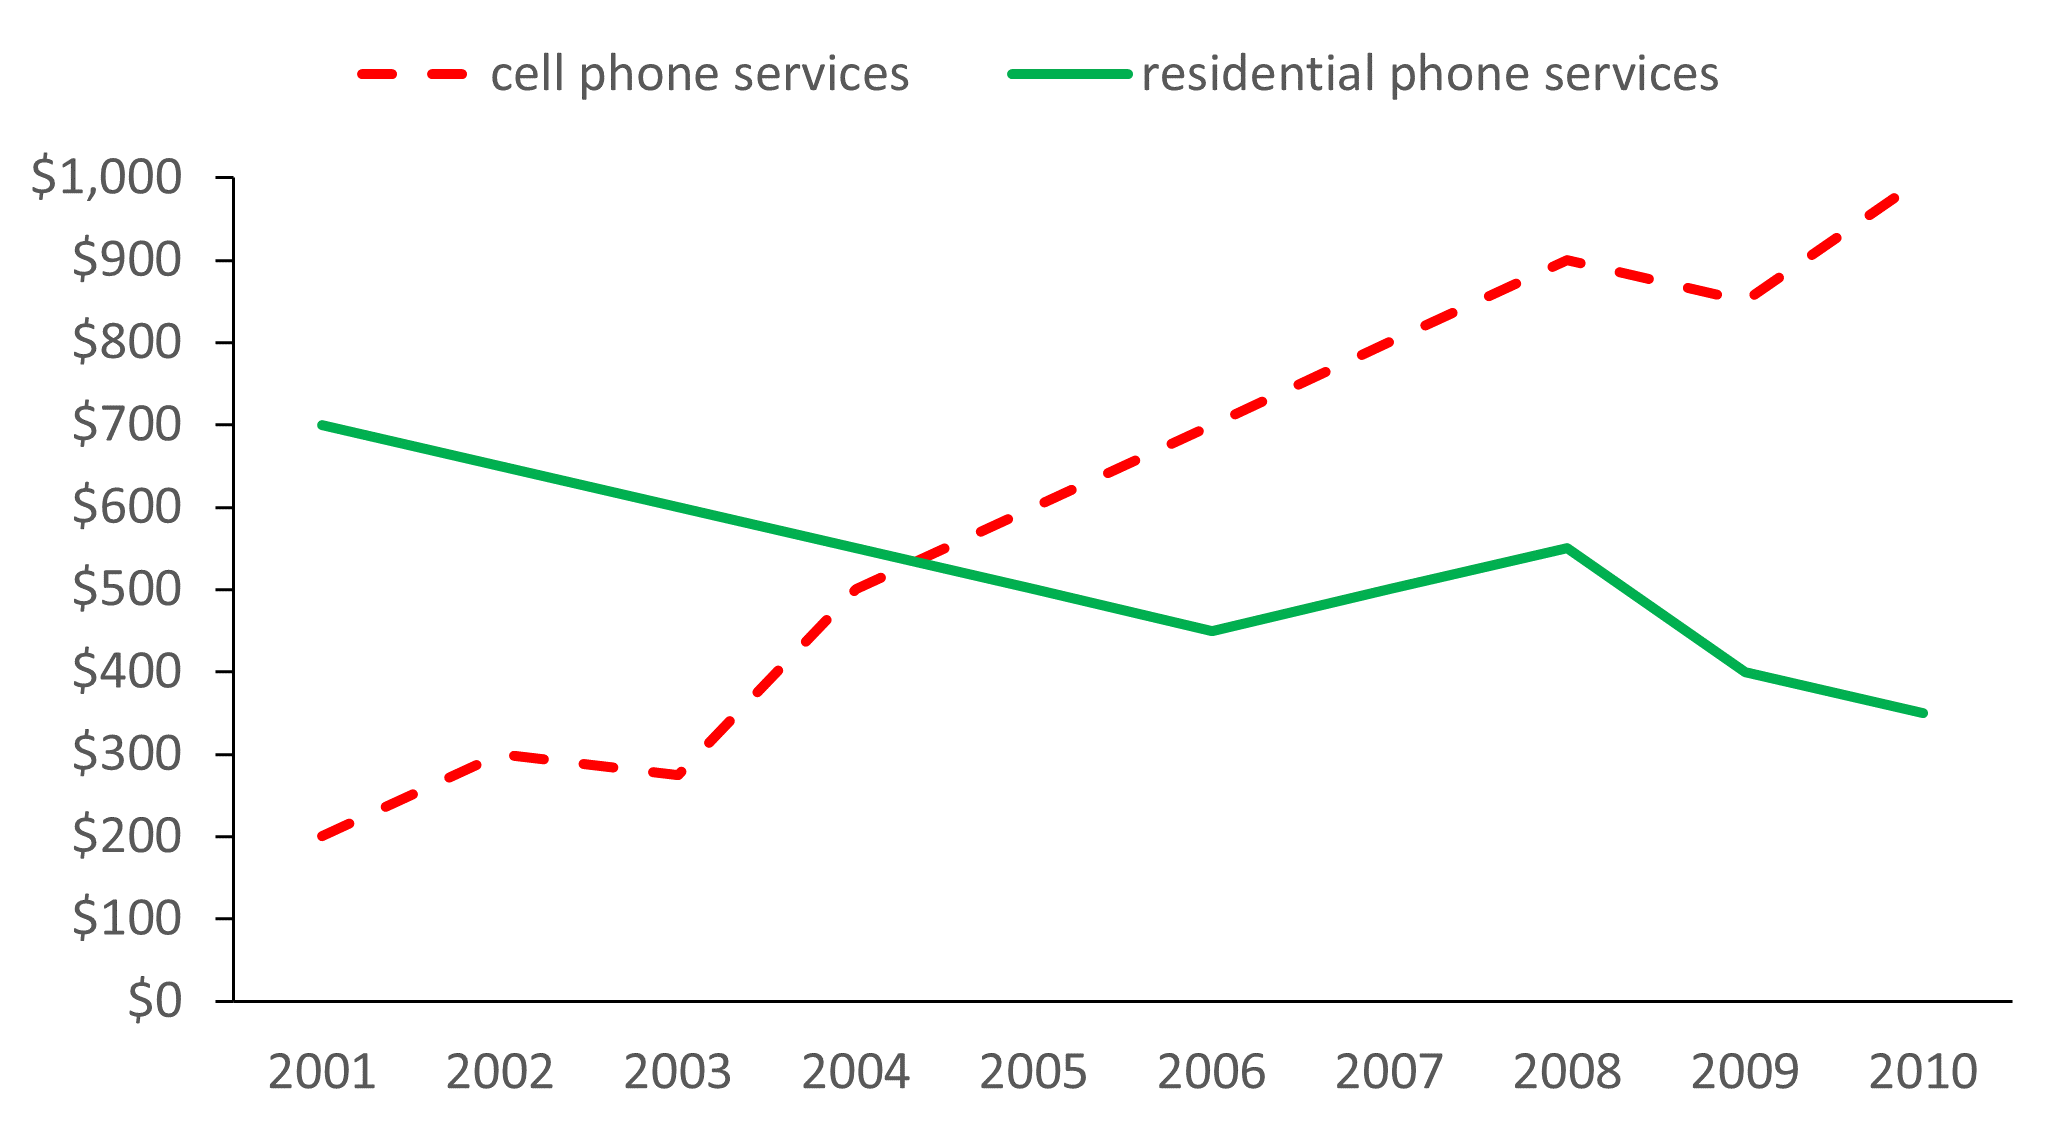
\includegraphics[width=6in]{Template-Fig-1.png}
  \tagmcend
 \tagstructend

	\caption{This is the caption text.}
	\label{fig:cellphone}

\end{figure}
 \tagpdfparaOn
If there was a corresponding data table in the same report, the following could be used: “Chart showing an upward trend over time; refer to the data table on this page for specific details.”
 

%%%%%%%%%%%%%%%%%%%%%%%%%%%%%%%%%%%%%%%%%%%%%%%%%%%%%%%%%%%%%%%%%%%%
%   Please use the techpubs BibTeX style when compiling bibliography to format your .bib / .bbl file appropriately.
% PLEASE NOTE THESE INSTRUCTIONS
% Examples are also provided here. Alternative formats can be used with permission from the NIST Research Library.
% Authors shall choose between Numeric (“[1]”) OR Named with no spaces (“[SP800-300]”) when numbering references. 
% Authors shall verify all references before submitting the document for publishing. This includes:
	% Checking validity of any DOI or URLs
	% Confirming the reference is the most current version/edition available (unless intentionally citing an older version)

%%%%%%%%%%%%%%%%%%%%%%%%%%%%%%%%%%%%%%%%%%%%%%%%%%%%%%%%%%%%%%%%%%%%
 \pagebreak
\tagpdfparaOff \tagstructbegin{tag=H1}
 \tagmcbegin{tag=H1}
\section*{References}
\tagmcend
 \tagstructend
\addcontentsline{toc}{section}{References}
 \tagpdfparaOn
\bibliographystyle{techpubs}
\bibliography{References}
 

%%%%%%%%%%%%%%%%%%%%%%%%%%%%%%%%%%%%%%%%%%%%%%%%%%%%%%%%%%%%
% Appendix section change for appendix package
%%%%%%%%%%%%%%%%%%%%%%%%%%%%%%%%%%%%%%%%%%%%%%%%%%%%%%%%%%%%
\titleformat{\section}{\normalsize\bfseries}{\appendixname~\thesection.}{0.3em}{}
\titleformat{\subsection}{\normalsize\bfseries}{\appendixname~\thesubsection.}{0.3em}{}
\titleformat{\subsubsection}{\normalsize\bfseries}{\appendixname~\thesubsubsection.}{0.3em}{}
\titleformat{\paragraph}{\normalsize\bfseries}{\appendixname~\theparagraph.}{0.3em}{}
%%%%%%%%%%%%%%%%%%%%%%%%%%%%%%%%%%%%%%%%%%%%%%%%%%%%%%%%%%%%
% Begin appendices
%%%%%%%%%%%%%%%%%%%%%%%%%%%%%%%%%%%%%%%%%%%%%%%%%%%%%%%%%%%%
\newpage
\begin{appendices}
\tagpdfparaOff \tagstructbegin{tag=Sect} %start sec
\tagstructbegin{tag=H1}
 \tagmcbegin{tag=H1}
\section{Selected Bibliography}
\label{app:bib}
\tagmcend
 \tagstructend
  \tagpdfparaOn
OPTIONAL. Additional sources of information not referenced in the text.  Do not include if the Reference section is a complete list.
 
 
\tagpdfparaOff \tagstructbegin{tag=H2}
 \tagmcbegin{tag=H2}
\subsection{Heading 2}
\tagmcend
 \tagstructend
  \tagpdfparaOn
Example of an Appendix Heading 2
  
  
 \tagpdfparaOff \tagstructbegin{tag=H3}
 \tagmcbegin{tag=H3}
\subsubsection{Heading 3}
\tagmcend
 \tagstructend
 \tagpdfparaOn
Example of an Appendix Heading 3


\tagpdfparaOff \tagstructbegin{tag=H4}
 \tagmcbegin{tag=H4}
\paragraph{Heading 4}
\tagmcend
 \tagstructend
 \tagpdfparaOn
Example of an Appendix Heading 4

 \newpage
 \tagpdfparaOff \tagstructbegin{tag=H1}
 \tagmcbegin{tag=H1}
\section{List of Symbols, Abbreviations, and Acronyms}
\label{app:abbr}
\tagmcend
 \tagstructend
 \tagpdfparaOn
OPTIONAL, if more than five symbols, abbreviations, and/or acronyms are used in a report that are not readily recognized as a standard in the field. Do not include symbols, abbreviations, and/or acronyms that are commonly used in the field of the target audience.


\begin{description}
\item[Abbreviation/Acronym/Symbol] Definition.
\item[Abbreviation/Acronym/Symbol] Definition.
\item[Abbreviation/Acronym/Symbol] Definition.
\end{description}

\newpage
 \tagpdfparaOff \tagstructbegin{tag=H1}
 \tagmcbegin{tag=H1}
\section{Glossary}
\label{app:gloss}
\tagmcend
 \tagstructend
 \tagpdfparaOn
OPTIONAL. List of terms defined and explained to facilitate a reader’s comprehension of the report. Begin each definition with a capital letter and end it with a period.
Use examples and instructions below when developing your glossary.
\begin{description}[leftmargin=40pt]
\item[Term 1]  test

~Original definition with no reference needed.

\item[Term 2] Original definition with a note.
\textit{Note:} Single note for a definition.
% Notes are optional and provide document-specific context. %

\item[Term 3] Definition that is copied exactly as it appears in the referenced source. \cite{1806-09936}

\textit{Note1:} First of multiple notes for a definition.

\textit{Note2:} Second of multiple notes.

% When a term/definition is copied exactly as it appears in another publication, include the [Reference] tag for that source at the end of the definition. All [Reference] tags in the Glossary must appear in the References section.
% Use the format above if multiple notes are included for a definition.
\item[Term 4] Definition from another source that is modified. \cite{1806-09936}, adapted
% Term with a definition adapted (modified) from another source.
\item[Term 5]~Definition. \cite{1806-09936}

~Definition. \cite{SP80053r4}
% Some terms may have multiple definitions.
\item[Term 6 (acronym)] Original definition with no reference needed.
% If your term also has an acronym, list it in parentheses here and ensure the acronym is specified in the “List of Symbols, Abbreviations, and Acronyms” appendix.

\item[Term 7] See Term 1.
%Some terms may be synonyms that direct the reader to another term (or terms) in this glossary. Please use discretion if considering whether to add terms like this. 
\item[Term 8] Original definition with no reference needed.

See also Term 1.

%If a defined term is closely related to (but NOT synonymous with) another term in this glossary, a “See also” statement can be included below the definition.

\end{description}

\newpage
 \tagpdfparaOff \tagstructbegin{tag=H1}
 \tagmcbegin{tag=H1}
\section{Index}
\label{app:index}
\tagmcend
 \tagstructend
 \tagpdfparaOn
OPTIONAL. Alphabetical listing of all major topics discussed in a report. An index cites the page or location where the topic can be found. The arrangement and level of detail of the index are determined by the structure of the report, its target audience, and use.
%\printindex%

\newpage
  \tagpdfparaOff \tagstructbegin{tag=H1}
 \tagmcbegin{tag=H1}
\section{Change Log}
\label{app:log}
\tagmcend
 \tagstructend
 \tagpdfparaOn
REQUIRED FOR UPDATES AND REVISIONS. If this report is an update, revision, or new edition of a previously published report, briefly state the changes made and the date of changes. Some examples of how to list changes made are: \\

In a table: 
\begin{table}[H]
\tagpdfparaOff \tagstructbegin{tag=Table}
 \tagmcbegin{tag=Table}
\begin{tabular}{|l|l|l|l|}
\hline
Date & Type of Edit & Change & Location \\ \hline
     &              &        &          \\ \hline
     &              &        &          \\ \hline
     &              &        &          \\ \hline
\end{tabular}
\tagstructend
 \tagmcend
\end{table}
\tagpdfparaOn
Or an informative sentence:

\tagstructbegin{tag=Div}
\tagmcbegin{tag=Div}
\begin{tcolorbox}%[before upper=\tagpdfparaOn]
Page 37, line 5 reads cosine of the angle, but should read sine of the angle.
\end{tcolorbox}
\tagmcend
\tagstructend

Or a narrative and accompanying bulleted list:

\vspace{12pt}
In May 2022, the following changes were made to the report:
\begin{itemize}
\item Abstract –provides direct information on the key establishment schemes (DH, MQV) and the underlying mathematics structure (discrete logs on finite field, elliptic curve).
\item Section 3.1 – Added definitions of assumption, binding, bit string, byte, byte string, destroy, key-establishment pair, key-wrapping key, trusted association; removed definitions on assurance of identifier, initiator, and responder.
\end{itemize}

\end{appendices}

\end{document}
